\documentclass[12pt,epsfig]{article}
\usepackage{fullpage}
\usepackage{epsfig,psfig}
\begin{document}
\pagestyle{plain}

\title{}
\thispagestyle{plain}


\section{General pContainer}

pContainers are the parallel counterparts of STL containers, and other
useful sequential data structures(eg. graph). To serve as
parallel/distributed data structure, a pContainer provides
semi-random/random access to each element in the data structure across
the machine. It also hides the data distribution information from the
user. Viewing from outside it is exactly the same as a sequential
container, and sequentially consistent in terms of the computation.

\subsection{Data Distribution Object}
Data distribution is a feature of the pContainer. Each pContainer
is associated with a specific distribution object. The distribution
has the information and functionality necessary to locate and move
elements of a pContainer across the machine.

\subsubsection{Partition, Mapping, Distribution}
A distribution is determined by data partitioning and mapping. A
partition is a decomposition of the elements in a sequential container
into disjoint sets. It can be generated using algorithms available in
STAPL toolbox, or provided by the user directly. It is a logical
arrangement of the data, not necessarily related with the machine
topology. A mapping is a logical placement of a partition onto the
machine. It can be computed based on machine topology using STAPL
tools, or designated by the user. The result of mapping a partition
onto the machine is a distribution. The user can also pre-define a
distribution, for example storing decomposed data into files on each
computation node.


\subsubsection{Element Location}
After data is distributed onto each computation node, an important
functionality of the distribution object is to locate remote data
items efficiently. This is done in a semi-random/random fashion based
on the specification of the sequential container. For example, to find
a data item in a parallel linked list, first we randomly locate the
processor it resides on, then we access sequential the linked list to
find it.

To facilitate the element location, an ElementLocator object is
associated with the Distribution.The ElementLocator finds the
location of a data element given its unique description, eg. a global
index for a pVector, or a global ID for a pGraph.  Element Location is
done in a distributed fashion by storing on each processor an element
location cache. The cache is similar to a distributed hash table, and
can be directly accessed from any processor. This solution is efficient
and scalable in terms of both memory and performance.


\subsubsection{Load-balancing/Re-distribution}
For some applications, the data layout of the container changes as
data elements are added, migrated or deleted. It can result an
imbalanced workload among processors and inefficient parallel
computation. Hence another functionality a Distribution provides is
load-balancing/redistribution. The work load on each processor is
checked periodically; If the imbalance ratio surpass certain
threshold, a re-distribution could be performed to restore the
balance. This process involves not only the pContainer, but also the
associated pRanges and the runtime system.

\begin{figure}[t]
\renewcommand{\baselinestretch}{1.}
\normalsize
\begin{center}
\includegraphics[height=2.5in,trim=0 20 0 0]{fig0.eps}
\end{center}
\caption{pContainer layout}
\label{fig:fig0}
\end{figure}

\subsection{User interaction with the Distribution of the pContainer}

The user of the pContainer can interact with the data distribution in
various ways. The three main steps in building a pContainer are data
partitioning, mapping and distribution. Any of these steps can be
performed using predefined methods available in STAPL or functions
provided by the user. For example the user can specify a uniform or
non-uniform partition and distribution or can use the STAPL scheduling
toolbox to compute a more efficient one.

When there are no dependencies among the data in the pContainer
simple partitioning strategies can be used. In cases when there are
precedence constraints among the data, which is represented by a Data
Dependence Graph (DDG) corresponding to the algorithm, the user can
select from a list of scheduling algorithms (STAPL scheduling toolbox)
to compute the partitioning and mapping of the computation onto the
multiprocessor machine.

\subsection{STAPL Scheduling Tool Box}
Currently there are a number of scheduling and mapping algorithms
available in the toolbox. For scheduling/partitioning, the algorithms
assume infinite/finite number of processor, with homogeneous
connection topology and computation power on each node. For mapping,
the algorithms assume finite number of processors, with
homogeneous/heterogeneous machine topology. Combining the scheduling
and mapping algorithms, the toolbox can produce distributions for the
pContainer to use.


\section{pGraph container}

Parallel graph is one of the parallel containers provided by
STAPL. Graph data structure is used widely in applications and some of
them work on large graphs which require an efficient distributed
implementation.  STAPL pGraph would be the ideal choice for these
problems. Parallel graph provides all the functionality of a
sequential graph. pGraph is used extensively by a number of projects
like ASCI[ref] and OBPRM[ref] and other components of STAPL like
pRange. These applications require highly scalable data structures and
pGraph was designed with this in mind.

A parallel graph is composed of a number of sequential graphs each of
them residing in one thread of execution. The pGraph could be
partition into these individual pieces through the user input
information or through a partition algorithm provided by STAPL.The
user can specify (build) the pGraph in a number of ways. It can be
specified in a sequential fashion in the form of a single file and
pGraph will automatically distribute the vertices in the graph
among available processors. If the user has already partitioned the
graph then it could be specified in a distributed fashion (like in a
number of files).  After the pGraph was distributed we have the option
to redistribute if necessary. The redistribution of the pGraph could be
done by the STAPL runtime or could be initiated by the user.


\subsection{The pGraph inheritance diagram}


STAPL is a highly modular library and pGraph is designed with the same
philosophy in mind. This allows the user to build new modules on top
of the existent one. We have identified the main characteristics for
a graph data structure as being the fact that is directed or
undirected, weighted or unweighted and with multiple edges between two
vertices or not. Each of the above characteristics is represented in
our model by a class and the graph that the user will instantiate is a
composition of these classes. Figure 1 and 2 describe this composition
model:

\begin{figure}
    \epsfig{figure=fig1.eps}
    \caption{pGraph components}
    \label{fig:fig1}
\end{figure}
\begin{figure}
    \epsfig{figure=fig2.eps}
    \caption{pGraph Inheritance}
    \label{fig:fig2}
\end{figure}

For example composing the pGraph from DirectedGraph, WeightedGraph and
Multi classes the user will have access to methods related with the
fact that the graph is directed(GetSuccessors, GetPredecessors),
weighted(GetEdgeWeight) and has multiple edges between two vertices.



\subsection{pGraph distribution}

PGraph data structure needs to maintain various bookkeeping information.
When a graph is distributed we need to find the location of a
particular element (eg. vertex) efficiently. This is the
responsibility of the graph distribution. The graph distribution
maintains a scalable distributed table which keeps the location of all
the vertices in the graph. Looking for an element in this table is a
two step process. Given a unique ID of the vertex (called VID) a hash
function is used first to find the processor which holds the
information about this VID. Then this processor is queried to find the
actual location of the vertex. Adding, removing, migrating and finding
a vertex in the graph could be done with the same asymptotic
complexity of a sequential graph and by using same asymptotic amount
of storage as the sequential graph.

\subsection{Ghost vertices}
PGraph needs to keep track of information that extends across
processor boundaries. In a pGraph there can be edges between
vertices residing in different processors. We deal with this case by
creating a 'ghost vertex'. Ghost vertices are images of the remote
vertices in the local processor. For example consider two vertices A
and B of a graph with an edge between them. If A and B are placed in
different processors a ghost vertex with information about the other
vertex is placed in each processor and a corresponding edge is added
between the real vertex and the ghost vertex. The sequential graph and
its parallel equivalent in shown in Fig 3.  


\begin{figure}
    \epsfig{figure=fig3.eps}
    \caption{Ghost nodes}
    \label{fig:fig1}
\end{figure}

Here A' and B' are the ghost vertices corresponding to A and B. Ghost
vertices act as a cache of information present in the real vertex. The
validity of the cached information has to be kept track of and the
cache has to be updated when required. In a graph data structure most
of the communication between vertices is between neighboring vertices
through the connecting edge. Keeping cached information in the form of
ghost vertices takes advantage of this characteristic and helps in
saving the time spent in retrieving remote information.

\subsection{pGraph prange}

The data inside pGraph can be accesed trough various methods like
DFS/BFS and also trough its associated pranges. For the graph data
structure there are two pranges: one that iterates trough vertices
of the pGraph and one that iterates trough the edges. 

\subsection{pGraph algorithms}

STAPL will provide generic parallel graph algorithms.  Sequential
graph algorithms like depth and breadth first search, strongly
connected components, topological sort and shortest paths can be
performed on pGraph. Next step in pGraph development is to
come up with efficient parallel counterparts for these
algorithms. Other algorithms like Euler tour, parallel graph
traversals would also be included in the future.

%\subsection{Status}
%At this moment we have most of the graph data structure implemented. A
%number of graph algorithms have already been implemented or are in the
%process of getting implemented.  

\end{document}
